% MediSense-Cardio -- journal manuscript (Physiological Measurement, IOP), REBUILT 2026-11-14 from results/FINAL_NUMBERS.md (sections 1-10.10).
% Replaces main.tex + sections/*.tex (the 2026-09-25 scaffold: 50 records, first sweep). Those files are kept unchanged and are out of date.
% Every number is taken from results/FINAL_NUMBERS.md; the numbers listed in its section 8 are never quoted.
% Not compiled locally (no LaTeX here). Upload docs/journal/ to Overleaf as a NEW project; main document = main_v2.tex; pdfLaTeX; BibTeX.
% Before submission: port to IOP iopart (optional), Harvard author-year is already used (natbib/apalike). Placeholders: title, authors, funding.
% Thresholds called "pre-set rules" are the team's proposal and NOT approved by the guide.

\documentclass[11pt,a4paper]{article}
\usepackage[margin=2.3cm]{geometry}
\usepackage[T1]{fontenc}
\usepackage{lmodern,microtype}
\usepackage{amsmath,amssymb}
\usepackage{graphicx,booktabs,array,tabularx}
\usepackage{xcolor}
\usepackage[authoryear,round]{natbib}
\usepackage{url}
\usepackage{setspace}
\usepackage[hidelinks]{hyperref}
\usepackage{caption}
\captionsetup{font=small,labelfont=bf}
\setstretch{1.1}

\newcommand{\todo}[1]{\textcolor{red}{\textbf{[TODO: #1]}}}
\newcommand{\bpm}{\,bpm}
\newcommand{\ms}{\,ms}
\newcommand{\mV}{\,mV}

\title{From a photographed paper ECG to what a patient is told: which image damage breaks which measurement, and which measurements are safe to show\\[2pt]
\large\textit{[working title -- to be confirmed]}}
\author{\todo{author names, affiliations, corresponding author e-mail}}
\date{}

\begin{document}
\maketitle

\begin{abstract}
\noindent\textbf{Objective.} To measure how photographic damage of a paper ECG propagates through a fixed open-source digitizer into heart rate and interval measurements, to test whether a reliability check can warn the user, and to decide for each measurement separately whether it is safe to show.

\noindent\textbf{Approach.} Open-ECG-Digitizer (commit 97a15087) was used unchanged on PTB-XL recordings drawn as 25~mm/s, 10~mm/mV pages, damaged by six controlled types at five levels, on competition captures (140 recordings, 9 capture types), and on the team's own phone photographs of pages shown on a screen. All rules were written before the result was seen and each test was run once; the results are labelled pre-specified, exploratory or post hoc. A traffic light was computed from 15 features of the digitized signal and frozen before real data were scored. A page-straightening step was confirmed on new photographs. Heart rate, PR interval, frontal QRS axis, QT interval, QRS duration and P- and T-wave amplitude were each validated against 12SL values from PTB-XL+.

\noindent\textbf{Main results.} On 99 held-out recordings, worst-level low resolution and blur gave a wrong heart rate (more than 5\bpm\ from the reference) in 47/99 (47.5\%) and 17/99 (17.2\%) pages; JPEG, brightness, faded grid and rotation did not, but 16$^\circ$ rotation produced no output on 19/99. A score from the picture alone was at chance inside a damage level (AUC 0.52 and 0.48); the digitized-signal check reached AUC 0.926, and GREEN readings on competition captures were wrong in 2/917 (0.2\%). Straightening cut bad readings from 14 to 2 of 40 new photographs (exact McNemar $p=0.0005$; 64 to 21 of 120 in a simulation). PR interval and frontal axis met the pre-set rules for straightened photographs (typical error 12.0\ms\ and 4.4$^\circ$). QT interval, QRS duration and P- and T-wave amplitude did not: their typical errors looked small but slope and bias checks exposed compression and bias.

\noindent\textbf{Significance.} Safeguards for photographed-ECG tools can target low resolution, blur and page geometry, and should warn from the digitized output rather than the picture. Measurements should be shown only after their extremes have been checked. The study is limited to one digitizer, one phone and one screen.

\medskip
\noindent\textbf{Keywords:} electrocardiogram; ECG digitisation; image degradation; reliability check; false reassurance; validation
\end{abstract}

\section{Introduction}
Printed and photographed ECGs are read outside the clinic: a photo sent over a messaging app, a home-device printout, an upload to a service that explains the ECG in plain words. Such services first turn the image back into a signal. Open tools can now digitize paper ECGs at scale \citep{ref5,ref3,ref53}, and public data and challenges have driven progress \citep{ref1,ref2,ref4}, building on classical image-processing work \citep{ref6,ref9}. Digitizers are usually validated on clean scans, whereas patients send tilted, blurred and low-resolution photographs.

Three questions are asked. \textbf{Q1:} which kinds of photo damage make a measurement wrong? \textbf{Q2:} can a reliability check warn the user, and from what: the picture or the digitized signal? \textbf{Q3:} which individual measurements can be shown at all? The third question matters because a measurement with a small average error can hide large errors where they matter most, such as a long QT or a wide QRS complex, and a falsely reassuring number is worse than no number.

The closest published work studies the robustness of digitizers to image damage \citep{ref54} and adds a vision-language quality-assurance module \citep{ref55}. This study differs in three ways: the digitizer is fixed and unmodified; each clinical measurement is judged separately against reference values under rules written down before the test; and the user-facing output is designed so that an unreliable result is never presented as reassuring.

\section{Related work}
\textbf{Digitization.} Early methods removed the grid, thresholded the trace and rescaled pixels to millivolts \citep{ref6,ref9}. The Moody PhysioNet Challenge 2024 asked teams to digitize and classify ECG images \citep{ref2}, supported by ECG-Image-Kit, which draws pages from recordings with realistic artifacts \citep{ref1}; a paired database of real captures followed \citep{ref4}. Open-ECG-Digitizer \citep{ref5}, ECGtizer \citep{ref3} and the winning Challenge entry \citep{ref53} are open pipelines.

\textbf{Quality assessment and abstention.} Most quality work scores ECG \emph{signals} \citep{ref12,ref13,ref14}. Selective prediction and deferral \citep{ref23,ref24} let a system decline to answer; a clinician study found that abstention reduced the effect of automation bias overall but increased missed problems \citep{ref26}. This study therefore makes no claim that a warning helps patients.

\textbf{Plain-language explanation.} Patient-facing explanations from language models are studied \citep{ref33}. Here no free text is generated: every sentence shown comes from a fixed list checked by a wording checker.

\section{Methods}

\subsection{Study design and discipline}
Every analysis has a rule log entry written before the run (\texttt{docs/plan/analysis\_plan\_changes.md}). Results are labelled \emph{pre-specified} (rule and pass/fail wording written before the result existed), \emph{exploratory} (the idea came after earlier data had been seen) or \emph{post hoc} (done to understand a result). The word ``confirmed'' is used only for tests whose rule was fixed before new data existed. Tests on sealed sets were run once, with guards in the code. Negative results are reported as measured. Calibration of a measurement was allowed to add an offset but never to rescale, because rescaling shrinks values toward the mean and hides errors.

\subsection{Data}
Recordings are from PTB-XL \citep{ref45}: 21,799 ten-second 12-lead records; pages are drawn from the 100\,Hz version. Reference interval and axis features are from PTB-XL+ \citep{ref46}, which provides measurements from two commercial algorithms (12SL and Glasgow). Subsets were fixed in advance with a random seed (Table~\ref{tab:sets}). The reference heart rate is measured by the same code on the recording the page was drawn from; a recording is \emph{reference-uncertain} when its 100\,Hz and 500\,Hz versions disagree by more than 5\bpm\ (20 of 150).

\begin{table}[ht]
\caption{Data sets. Seeds were fixed before any result.}
\label{tab:sets}
\centering\small
\begin{tabular}{p{4.6cm}p{2.2cm}p{6.4cm}}
\toprule
Set & Size & Use \\
\midrule
First 50 recordings & 50 (1,550 images) & Development; damage sweeps \\
New 100 recordings & 100 (1,300 images) & Held-out replication; safeguard training \\
Competition captures & 140 rec.\ $\times$ 9 types & Real captures (1,260 images) \\
Own phone set 1 & 30 pages, 60 photos & Frozen-model evaluation \\
Own phone set 2 & 20 pages, 40 photos & Confirmation of straightening \\
Development 1,000 + 100 fresh & 1,100 + 100 & Method development for QT, QRS, axis \\
Sealed set G & 100 pages, 40 photos & QRS/QT third attempt; P/T amplitude \\
\bottomrule
\end{tabular}
\end{table}

\subsection{Pages, damage and real captures}
Pages are drawn with a patched copy of ECG-Image-Kit \citep{ref1} at 25\,mm/s, 10\,mm/mV and 200\,dpi, so that one pixel equals 5.08\ms\ in time and 0.0127\mV\ in amplitude; page size is 2200$\times$1700 pixels with the standard three rows of four leads plus a long lead~II strip. Six damage types are applied at five levels each: Gaussian blur (kernel 3 to 21), rotation (2 to 16$^\circ$), JPEG compression (quality 50 to 3), low resolution (shrink factor 0.75 to 0.15, then enlarge), a left-to-right brightness ramp (0.15 to 0.75), and a faded grid (contrast pulled toward the mean, 0.15 to 0.75). Real captures are the public competition images (print-scan colour and black-and-white, phone photographs of print and of a screen, stained, extensively damaged, mouldy scans; 9 types) and the team's own photographs of pages shown on a laptop screen, taken straight on and from about 30$^\circ$.

\begin{figure}[ht]
\centering
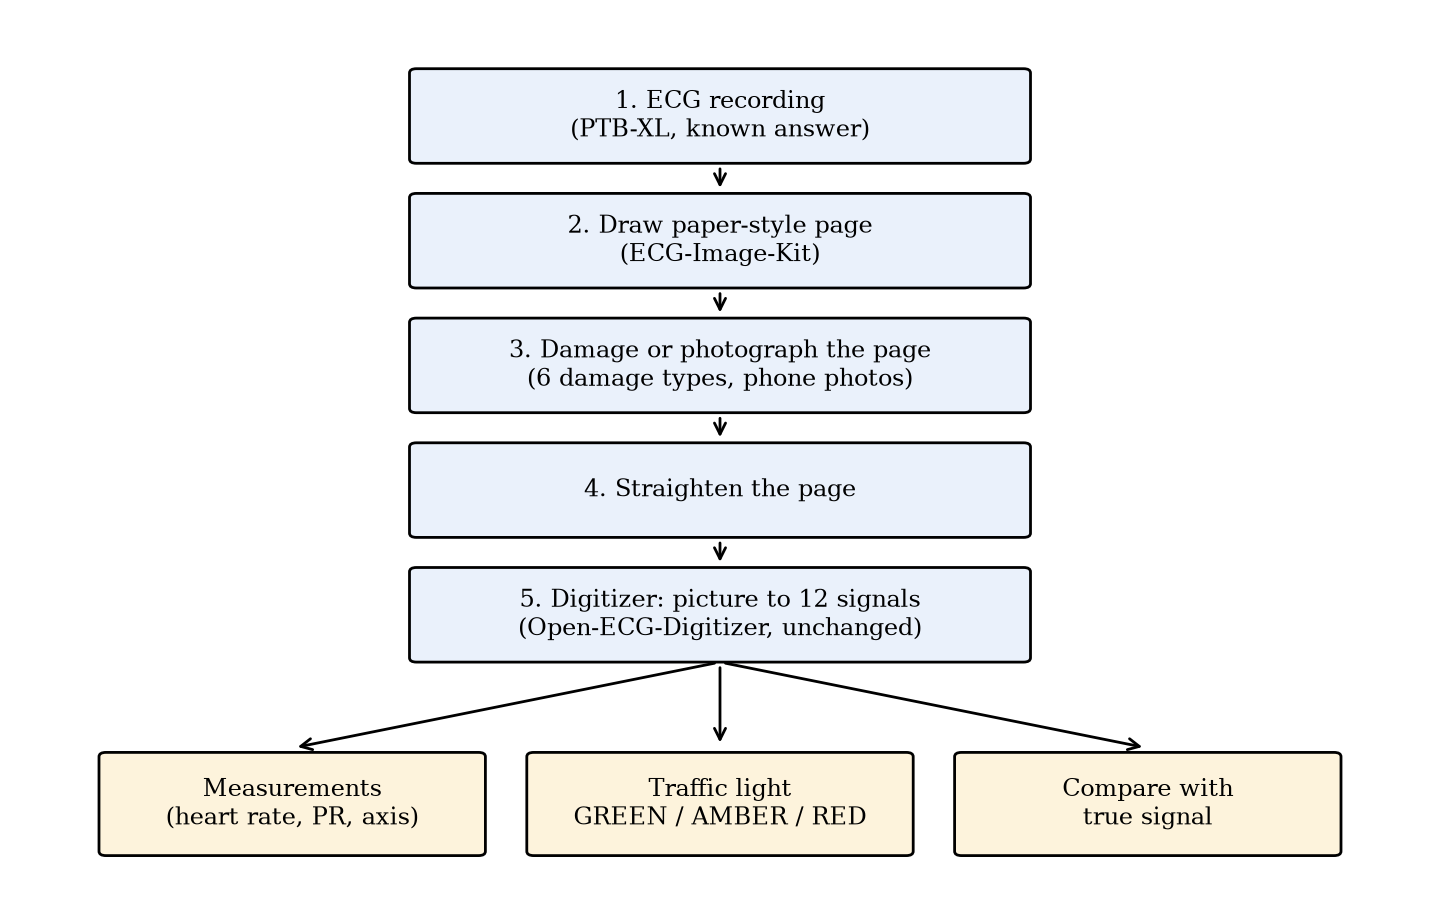
\includegraphics[width=0.7\textwidth]{figures/fig_pipeline.png}
\caption{The method as a flow of steps.}
\label{fig:pipeline}
\end{figure}

\subsection{Digitizer and heart rate}
Open-ECG-Digitizer \citep{ref5} was used unchanged (commit 97a15087, published weights, one settings file for every run). A U-Net finds trace and grid, a Hough transform estimates tilt, grid spacing gives pixel size, and the trace is read out at 1,000\,Hz in microvolts; unreadable leads are returned as missing. The digitizer is slightly non-deterministic. Heart rate is the mean of $60/RR_i$ from R-peaks found by NeuroKit2\footnote{\url{https://github.com/neuropsychology/NeuroKit}} on cleaned lead~II, for the reference and the digitized signal alike. A reading is \emph{wrong} if it differs from the reference by more than 5\bpm, and has \emph{no usable heart rate} if fewer than 3 beats are found; \emph{bad} means wrong or no usable heart rate.

\subsection{Statistics}
Rates carry Wilson 95\% intervals; because several images come from one recording, intervals for rates and AUC are obtained by resampling whole recordings (1,000 or 2,000 resamples). Paired binary comparisons use the exact McNemar test with Holm correction. Agreement uses Bland--Altman bias and limits. AUC measures how often a bad reading receives a higher risk than a good one. Cross-validation (5 folds, 10 repeats) keeps all images of a recording in one fold. Sample size follows Riley's criterion; with fewer than 100 wrong readings results are called descriptive.

\subsection{Reliability check}
Fifteen features are computed only from the digitized signal: share of readable lead~II samples, number of unreadable leads, mean completeness of the other leads, beat count, heart rate and its plausibility, RR variation (rr\_cv), maximum and minimum RR ratios, amplitude, high-frequency share, Einthoven consistency $\mathrm{RMS}(II-I-III)/\mathrm{RMS}(II)$, Goldberger consistency, and the agreement of beat counts across leads. A logistic regression with median imputation and standardization is trained once on the simulated 100 and frozen. AMBER starts at the 10th percentile of the scores of wrong readings in training (0.2585), RED at the lowest score above which at least half the readings are wrong (0.7823); fewer than 3 beats is RED; a guard turns GREEN into AMBER when a feature leaves its training range. The photo-quality comparator uses five picture scores (Laplacian variance, line skew, high-frequency share, contrast, blockiness).

\subsection{Straightening}
The page is found on an 800-pixel copy (Gaussian blur, Otsu threshold, closing and opening, largest contour of at least 12\% of the image, polygon approximation to four corners) and mapped by a perspective transform to 2200$\times$1700 pixels with cubic interpolation; a result is accepted when its aspect ratio is between 0.9 and 1.8. Variants tested: original, enlarge to 4,096 pixels, straighten, straighten and enlarge.

\subsection{Per-measurement validation}
PR, QT, QRS duration, P- and T-wave amplitude are measured from a median beat per lead with the authors' own code (QRS onset by a slope fraction of the maximum, T end by the tangent method, P onset by tangent; QRS duration also from a combined-lead activity curve). Frontal axis uses the net QRS deflection of the six limb leads by least squares. For each measurement the protocol was: development on original signals of 1,000 to 1,100 recordings with cross-validation and an offset-only calibration; one test on sealed pages; one confirmation on phone photographs; \emph{validated} only if all parts meet the pre-set rule (Table~\ref{tab:rules}). Measurements on which 12SL and Glasgow disagree strongly (P duration, T duration, ST amplitude) were not attempted: the reference cannot validate them.

\begin{table}[ht]
\caption{Pre-set pass rules (team proposal, not approved by the guide).}
\label{tab:rules}
\centering\small
\begin{tabular}{p{2.4cm}p{5.4cm}p{5.2cm}}
\toprule
Measure & Typical error / share within / bias & Extra conditions \\
\midrule
QT & 20 ms / 90\% within 40 ms / 10 ms & slope $\ge$0.8; tails (QT $\ge$450, $\le$350 ms) within 20 ms \\
QRS & 10 ms / 90\% within 20 ms / 5 ms & slope $\ge$0.8; tail (QRS $\ge$120 ms) \\
PR & 20 ms / 90\% within 40 ms / 10 ms & value for $\ge$90\% \\
Axis & median 10$^\circ$ / 90\% within 30$^\circ$ / 10$^\circ$ & category agreement $\ge$90\% \\
P amplitude & 0.03 / 0.06 / 0.015\mV & slope $\ge$0.8 \\
T amplitude & 0.05 / 0.10 / 0.03\mV & slope $\ge$0.8; sign agreement $\ge$90\% \\
\bottomrule
\end{tabular}
\end{table}

\section{Results}

\subsection{Which damage makes heart rate wrong (pre-specified)}
On the held-out 100 recordings at the worst level, only low resolution and blur gave many wrong heart rates (Table~\ref{tab:damage}, Fig.~\ref{fig:damage}); this held with and without the reference-uncertain recordings, and with all 148 reliable recordings (resolution 68/148 = 45.9\%, blur 25/148 = 16.9\%). At medium damage every type gave 1 to 6\% wrong, close to the clean page (3.0\%). Rotation did not give wrong readings; it gave no output on 19/99 pages. Paired against each recording's clean page, low resolution (median error 3.8 against 0.09\bpm) and blur (1.5 against 0.09\bpm) differed after Holm correction; JPEG, brightness and faded grid did not. A repeat run of 12 recordings (156 images) changed the bad label on none and gave heart rates within 1\bpm\ on 153 of 155; the first and second sweep differed in the number of unreadable images (163 against 30) for an unknown reason, so the second sweep is a repeat, not a replication.

\begin{table}[ht]
\caption{Wrong heart rate at the worst level, held-out 100 recordings.}
\label{tab:damage}
\centering\small
\begin{tabular}{lrll}
\toprule
Damage & Wrong & 95\% interval & No output \\
\midrule
Clean page & 3/99 = 3.0\% & 1.0--8.5\% & 0 \\
Low resolution (15\%) & 47/99 = 47.5\% & 37.9--57.2\% & 0 \\
Blur (21$\times$21) & 17/99 = 17.2\% & 11.0--25.8\% & 1/99 \\
Rotation (16$^\circ$) & 0/99 & 0.0--3.7\% & 19/99 \\
JPEG (quality 3) & 0/99 & 0.0--3.7\% & 0 \\
Brightness ramp (0.75) & 1/99 = 1.0\% & 0.2--5.5\% & 1/99 \\
Faded grid (0.75) & 3/99 = 3.0\% & 1.0--8.5\% & 0 \\
\bottomrule
\end{tabular}
\end{table}

\begin{figure}[ht]
\centering
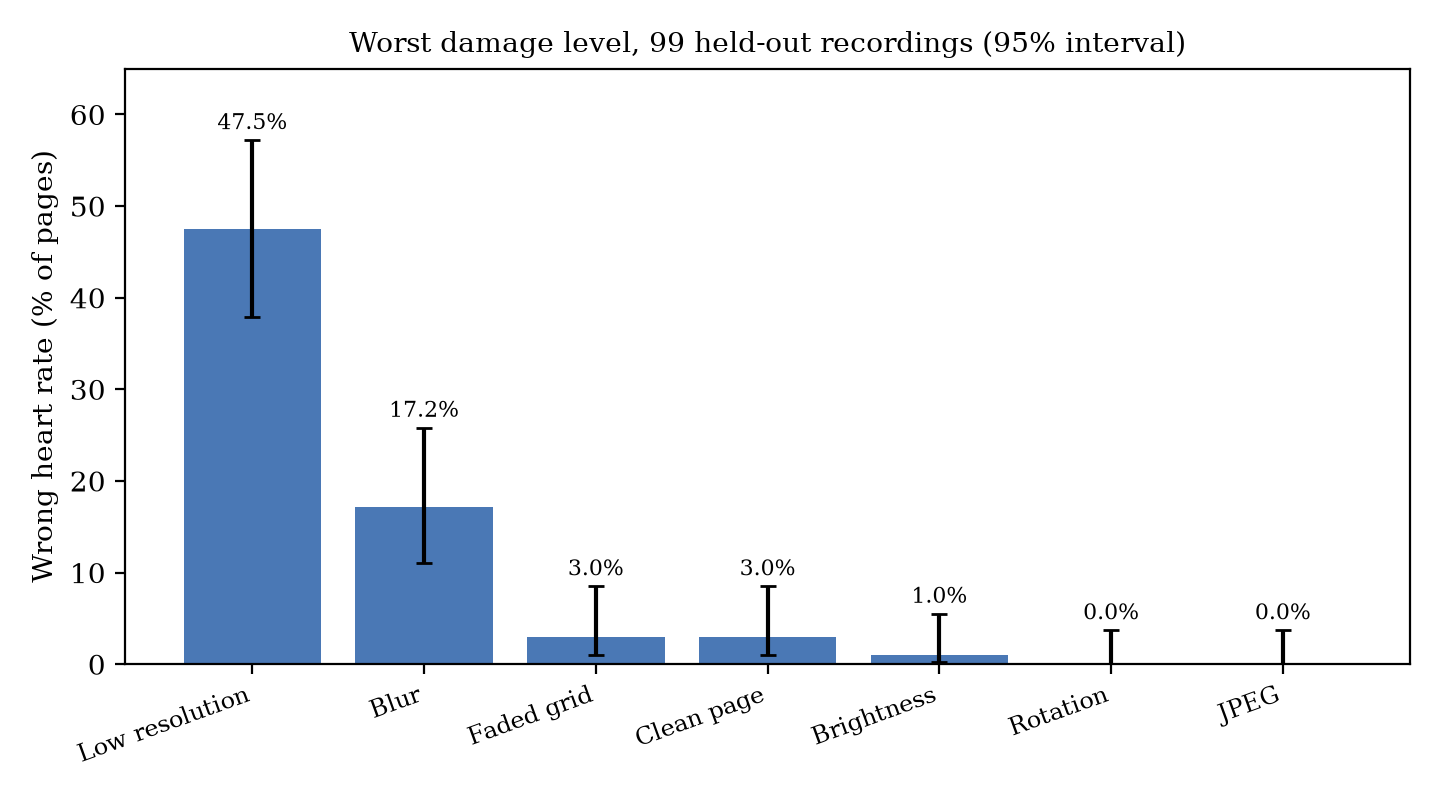
\includegraphics[width=0.75\textwidth]{figures/fig_wrong_by_damage.png}
\caption{Wrong heart rate at the worst damage level (95\% intervals).}
\label{fig:damage}
\end{figure}

\subsection{Waveform quality (exploratory)}
On clean drawn pages the digitized lead~II matched the true signal with median correlation 0.974, mean absolute error 0.0107\mV, root-mean-square error 0.0282\mV, gain error $-0.02\%$ and R-peak timing error 2.5\ms; R peaks were read about 0.080\mV\ too low. At the worst level blur reduced the correlation to 0.54 and low resolution to 0.65. The median aligned signal-to-noise ratio was 11.8\,dB on clean pages and 2.2 and 0.6\,dB at resolution and blur level~5; a low ratio goes with a wrong heart rate (AUC 0.828) but 9 images with acceptable ratio still had a wrong heart rate, so it is not a safe stand-alone check. On real captures the correlation fell from 0.99 (kit original) to 0.76--0.79 (print-scan), 0.71--0.73 (mould scans) and 0.47 (phone photos of print); for own photographs that were not straightened, angled shots had correlation 0.54 and a median gain error of $-48\%$ (set~1). Timing differences below 5 to 10\ms\ are not meaningful at this resolution.

\subsection{A picture-only warning fails; the digitized output works}
\emph{Pre-specified.} Five picture scores, trained on the first 50 recordings and scored once on the held-out 100, gave AUC 0.858 (0.81--0.91); an oracle told only the damage type and level gave 0.827 (0.77--0.90). Inside one damage type and level the detector was at chance (resolution level 5: 0.521; blur level 5: 0.476), it did not generalize to unseen damage types (0.78, 0.56, 0.37, 0.48 for resolution, blur, brightness, grid left out), and on real captures it scored 0.516 (0.46--0.57). The held-out set held 86 wrong readings, fewer than 100, so the verdict is inconclusive and the honest reading is negative.

\emph{Exploratory.} Fifteen features of the digitized signal gave AUC 0.926 (0.89--0.95), against 0.724 for the picture scores; inside resolution level~5 and blur level~5 the AUC was 0.873 and 0.892 against 0.481 and 0.432. Beat regularity alone gave 0.892 and agreement between leads 0.838. At the top-20\% flag level, right readings were flagged for 13\% of normal recordings but for 67\% (45/67) of readings on atrial fibrillation or flutter recordings: a truly irregular rhythm cannot be told from a failed read. Five beat detectors added no value (+0.005 against the required +0.02).

\subsection{Real captures (exploratory, post hoc)}
No capture type of the competition data was significantly worse than the clean kit page in wrong heart rate (all Holm $p>0.5$). The one large effect was no output for phone photographs of a screen: 53/140 = 38\% (30--46\%), against 1\% on the clean page ($p<0.001$). The clean page itself gave a wrong heart rate for 16/140 = 11\% of recordings: the digitizer drew the right waveform (median correlation 0.98) and the fault lay in a fragile one-number heart rate from raw beat finding on hard rhythms. Applying the same cleaning filter to the true and the digitized signal before beat finding cut wrong readings from 168 of 1,203 to 46 of 1,201; this correction was made after seeing the problem, so both versions are reported. Trained only on simulated damage and applied once, the output check reached AUC 0.923 (0.86--0.97) on 1,201 images with 46 wrong (descriptive; 0.64 with the original labels).

\subsection{Own phone photographs}
Set~1 (60 photos of 30 pages on a laptop screen): 6 had no usable heart rate and 14 a wrong one (20/60 bad); angled and small photos failed most (13 of 15). The photo detector did not predict failure (AUC 0.552, 0.32--0.80); the output check predicted a wrong heart rate with AUC 0.855 (0.71--0.96) on 54 photos with an output.

\subsection{Traffic light (exploratory)}
\begin{table}[ht]
\caption{Wrong heart rate by traffic light (images with an output). Intervals treat images as independent.}
\label{tab:light}
\centering\small
\begin{tabular}{llrl}
\toprule
Data & Light & Readings & Wrong (Wilson 95\%) \\
\midrule
Competition captures & GREEN & 917 & 2 (0.2\%, 0.1--0.8) \\
 & AMBER & 204 & 14 (6.9\%, 4.1--11.2) \\
 & RED & 82 & 30 (36.6\%, 27.0--47.4) \\
Own phone, set 1 & GREEN & 22 & 0 (0.0\%, 0--14.9) \\
 & AMBER & 15 & 1 (6.7\%, 1.2--29.8) \\
 & RED & 17 & 13 (76.5\%, 52.7--90.4) \\
\bottomrule
\end{tabular}
\end{table}
Frozen before any real data were scored, the light separated wrong readings (Table~\ref{tab:light}). If a missing output also counts as RED, RED holds 87 of 139 bad competition readings (62.6\%) and 84\% of all bad readings, and GREEN still holds 2 bad of 917. With fewer than 100 wrong readings the result is descriptive; GREEN is not a guarantee.

\subsection{Straightening (exploratory, then confirmed)}
On the first 60 photos, bad readings fell from 20 (original) to 12 (enlarge; Holm $p=0.0215$), 2 (straighten; $p=0.0001$) and 6 (both; $p=0.0087$); the fix was designed after seeing these photos, so this is exploratory. The confirmation used 40 photographs of 20 new pages with the rule fixed beforehand (Table~\ref{tab:fix}): newly bad 0, newly good 12, exact McNemar $p=0.0005$. Enlarging alone gave 13/40 bad and adding enlargement to straightening 3/40. No bad reading received GREEN (0 of 20 GREEN on originals, 0 of 32 on straightened photos). A simulation added afterwards used 120 phone photographs of 60 sealed pages made by a script (not a camera) with tilt, a screen edge, vignette, noise, and on random photographs blur, a shadow or a smaller page; the rule was fixed before the photographs existed and the test was run once. Bad readings fell from 64 to 21 of 120 (newly bad 5, newly good 48; exact $p=7\times10^{-10}$), from 13 to 5 of 60 straight shots and 51 to 16 of 60 angled shots; blur was helped least (19 to 10 of 35). On the straightened photographs GREEN had 71 readings with 1 wrong, AMBER 26 with 10 bad and RED 23 with 10 bad, so GREEN is not a guarantee. The two remaining bad readings belong to one page that the digitizer reads wrongly whatever the photo (66 against a true 58\bpm).

\begin{table}[ht]
\caption{Confirmation of the straightening fix, 40 new photographs.}
\label{tab:fix}
\centering\small
\begin{tabular}{lrr}
\toprule
 & Original photo & Straightened \\
\midrule
Bad readings & 14/40 & 2/40 \\
No usable heart rate & 4 & 0 \\
Wrong heart rate & 10 & 2 \\
Straight shots bad & 4/20 & 1/20 \\
Angled shots bad & 10/20 & 1/20 \\
Traffic light GREEN (bad among them) & 20 (0) & 32 (0) \\
\bottomrule
\end{tabular}
\end{table}

\subsection{Per-measurement validation (exploratory)}
\textbf{Standard method.} The NeuroKit2 wavelet delineation failed on the original signal already (typical error QT 36\ms, PR 78\ms, QRS 84\ms against 12SL), so the photo could not be blamed. The authors' median-beat methods gave the results in Table~\ref{tab:valid}.

\textbf{PR interval.} PR met the pre-set rule on held-out original signals (8.2\ms), held-out digitized pages (7.3\ms, 97\% within 40\ms) and 100 straightened phone photos (12.0\ms, 95\% within 40\ms; 91 of 100 with a value); without straightening only 67\% of photos gave a value. It holds only for rhythms in which 12SL finds a P wave: for atrial fibrillation or flutter, 6 of 99 held-out pages and 12 of 100 photos have no 12SL PR and were left out of the statistics, yet the method still produced a number for all 6 pages and 7 of 12 photos. In the demonstration PR is therefore hidden when rr\_cv exceeds 0.12 (caught all 6 pages and all 8 photos of such recordings, hid PR on about 15\% of normal-rhythm photos); this is a precaution calibrated on 14 cases, not a validated filter.

\textbf{Frontal axis.} Axis met the rule on 100 fresh pages (3.8$^\circ$, 99\% within 30$^\circ$) and 100 straightened photos (4.4$^\circ$, 95\% within 30$^\circ$, category agreement 92\%); not straightened it did not (87\% within 30$^\circ$; value on 82\%). One recording (12SL axis 148$^\circ$) was measured at $-95^\circ$ and $-91^\circ$ on its two photos; all 8 fresh left-axis pages were placed in the left category but the fresh test had no right-axis recording and on photos a right axis was matched in 0 of 4: right-axis detection is not shown to work.

\textbf{QT interval.} A first median-beat method gave 13.5\ms\ on digitized held-out pages with bias $+10.5$\ms, 0.5\ms\ over the limit, and 19.5\ms\ with 84\% within 40\ms\ on new photos. On fresh data a second attempt met the error rule on drawn pages (8.8\ms) but not on photos (14.9\ms, bias $-16.5$\ms, 86\% within 40\ms), and the slope of measured on 12SL QT was 0.68 to 0.69, below the limit of 0.7 set in advance for that attempt: a true QT of 350\ms\ or less was overestimated by 23 to 27\ms, which would make a short QT look normal. A third attempt (a combined-lead method, stricter slope 0.8 and tail rules) could not freeze a QT candidate and was not tested.

\textbf{QRS duration.} Three attempts failed. In the third, on 100 sealed pages the digitized-page test met the rule (5.5\ms, slope 0.87) but the original-signal check had slope 0.79 against 0.8, and the rule needed both; on 40 straightened photos the typical error was 6.2\ms\ but the bias $+15.4$\ms\ and the slope 0.74. In the second attempt recordings with a true QRS of 120\ms\ or more were read 42 to 47\ms\ too short, so a wide QRS would look normal. At 200\,dpi one pixel is about 5\ms, so a 10\ms\ rule is close to what a photograph can resolve.

\textbf{P- and T-wave amplitude.} Only the amplitude in lead~II was attempted. P amplitude met the rule on 100 sealed pages (original 0.013\mV, slope 1.04; digitized 0.012\mV, slope 0.99) but on 40 straightened photos the slope was 0.77 (bias $-0.014$\mV), so it is not validated; T amplitude reached a slope of at most 0.72 in development and was not tested. ST segment, P duration and T duration were not attempted.

\begin{table}[ht]
\caption{Validation against 12SL (typical error; slope on 12SL where checked; verdict).}
\label{tab:valid}
\centering\small
\begin{tabular}{llll}
\toprule
Measure & Test set & Typical error; slope & Verdict \\
\midrule
PR & held-out digitized pages & 7.3 ms & met \\
PR & photos, straightened & 12.0 ms & met \\
PR & photos, not straightened & 8.7 ms; 67\% with value & not met \\
Axis & 100 fresh pages & 3.8$^\circ$ & met \\
Axis & photos, straightened & 4.4$^\circ$ & met \\
Axis & photos, not straightened & 4.9$^\circ$; 82\% with value & not met \\
QT & fresh pages (attempt 2) & 8.8 ms; 0.69 & slope fails \\
QT & photos, straightened (attempt 2) & 14.9 ms & not met \\
QRS & 100 sealed pages, digitized & 5.5 ms; 0.87 & met (original: slope 0.79) \\
QRS & photos, straightened & 6.2 ms; 0.74 & not met \\
P amplitude & 100 sealed pages & 0.012 mV; 0.99 & met \\
P amplitude & photos, straightened & 0.014 mV; 0.77 & not met \\
T amplitude & development & slope 0.68 & stopped \\
\bottomrule
\end{tabular}
\end{table}

\subsection{Demonstration}
The local demonstration shows heart rate with the light; PR only under GREEN, a straightened page, a value of 50 to 400\ms\ and rr\_cv $\le0.12$; axis in degrees only under GREEN on a straightened page, never with a verdict word; and lists QT, QRS duration, P wave, T wave and ST segment as not measured by this tool. Every sentence comes from a fixed list checked by a wording checker and 19 automated tests, and a RED light or no output says nothing about the heart.

\section{Discussion}
Three findings stand out. First, the fixed digitizer is more robust than expected: only very low resolution and heavy blur broke the heart rate, and rotation produced missing output rather than wrong numbers. Second, the picture cannot say which pages will fail, whereas the digitized signal can, and the simplest effective fix on real photographs was geometric: finding and flattening the page. Third, validating measurements one by one showed that heart rate, PR and axis can be read from straightened photographs, while QT, QRS duration and P- and T-wave amplitude cannot yet be read safely.

The slope and tail checks matter. QRS duration had a typical error of 5 to 6\ms\ and a bias of $+15$\ms\ on photos; QT looked close on drawn pages while compressing short values toward the mean. A measurement judged only by its average error would have been accepted. These checks were fixed before the tests and not relaxed after a miss, because relaxing them would have produced a passing but misleading result. For the same reason the ST segment was not attempted: its commercial references disagree and its spread is under four pixels.

The traffic light adds a safety layer but also flags irregular rhythms, so RED does not mean a bad heart, and the PR guard shows how a measurement can still give a number where no P wave exists. The results do not show that the tool helps patients, and the clinician study on selective prediction warns that abstaining can increase missed problems \citep{ref26}.

\section{Limitations}
Damage is simulated on computer-drawn pages and the digitizer was trained on a similar generator; only one digitizer was studied. Phone results come from one phone and one laptop screen, photographing a screen and not paper, and the two photos of a page are not independent. Real captures hold fewer than 100 wrong readings, so those results are descriptive; several intervals treat images as independent and are optimistic. The reference heart rate depends on the beat finder and the sampling rate for 13\% of recordings. Interval references are commercial algorithms (12SL), not expert annotations, and the pass thresholds are the team's proposal, not approved by the guide. Methods were developed on 50 to 1,100 recordings with a small number of candidates and one offset each, which allows mild overfitting. The traffic light was trained on simulated damage and flags irregular rhythms more often. The sealed pages and photographs used for the QRS and QT attempts were reused for P- and T-wave amplitude (no P or T result had been seen; the methods were developed elsewhere). Only the straightening fix was confirmed in a test whose rule was fixed in advance; every other result is exploratory. The tool is a research prototype and not a medical device.

\section{Conclusions}
With a fixed open digitizer, only very low resolution and heavy blur made the heart rate wrong at a high rate; a picture-only score could not predict failure but a traffic light from the digitized signal flagged most bad readings; flattening the photographed page cut bad readings from 14 to 2 of 40 in a confirmed test; and measurement-by-measurement validation accepted heart rate, PR and axis for straightened photographs while rejecting QT, QRS duration and P- and T-wave amplitude. Future work should test other phones, paper and digitizers, use expert annotations, search for QT, QRS and P/T methods that pass the slope check, and study with clinicians whether the warning changes decisions.

\section*{Reproducibility and data availability}
All numbers are in \texttt{results/FINAL\_NUMBERS.md}; the rule log is \texttt{docs/plan/analysis\_plan\_changes.md}; a script recomputes 36 headline numbers from raw files (all match; it is a second script by the same author, and a second person's recheck of three numbers is still open). PTB-XL, PTB-XL+ and the competition image dataset are public. Code and the demonstration are in the project repository. \todo{repository link, funding statement, ethics statement (public data only), author contributions}

\bibliographystyle{apalike}
\bibliography{references}

\end{document}
